\section*{4 Proof of Theorem8}
Let $\Phi=\operatorname{TseitinBridge}(G,H,\phi)$ and let $e^*$ be an edge of $G$. We will show that $\operatorname{width}(\Phi\vdash\bar x_{e^*})>\ell-1$ for all such edges $e^*$. In fact, we will prove $\operatorname{width}(\Phi|_{x_{e^*}\mapsto1}\vdash\square)>\ell-1$, which is a slightly stronger statement.
We will use the game characterization of resolution width due to Atserias and Dalmau [2]. Given a CNF formula $F$, the $\ell$-bounded Atserias-Dalmau game played by two players, Prover and Delayer is defined as follows. A position in this game is a partial assignment $\alpha$ setting up to $\ell$ variables. The start position is the empty assignment. At position $\alpha$, Prover can either (1) forget some variables, i.e., replace $\alpha$ by some $\beta\subset\alpha$. Or, (2), if $|\operatorname{var}(\alpha)|\le\ell-1$, pick a variable $x\notin\operatorname{var}(\alpha)$ and query it; Delayer has to respond with a truth value $b\in\{0,1\}$, and $\alpha$ is updated to $\alpha\cup(x\mapsto b)$. The game ends if $\alpha$ violates a clause of $F$, in which case Prover wins. Delayer wins if she has a strategy to play indefinitely.
\begin{authorclaim}{Theorem9 (Atserias and Dalmau [2])}
Let $F$ be an unsatisfiable CNF formula. If Delayer has a winning strategy for the $\ell+1$-bounded game then there is no width-$\ell$ resolution refutation of $F$.
\end{authorclaim}
To show that $\operatorname{width}(\Phi|_{x_{e^*}\mapsto1}\vdash\square)>\ell-1$ we define a winning strategy for Delayer for the $\ell$-bounded game that ensures she never loses. Indeed, we will modify the game a bit: it is now played on $\Phi$ instead of $\Phi|_{x_{e^*}\mapsto1}$; the starting position is the partial assignment $x_{e^*}\mapsto1$; Prover can never forget $x_{e^*}$ but is now allowed partial assignments up to size $\ell+1$. That is, he can query a new variable provided $|\operatorname{var}(\alpha)|\le\ell$. It is easy to see that if Delayer wins this modified game, she wins the original one, too. Since $\Phi=\operatorname{TseitinBridge}(G,H,\phi)$, we can easily rephrase the rules of the game in terms of sets of edges instead of partial assignments:
\begin{quote}
\textbf{The Atserias-Dalmau, Graph View.} A position of the game is described by two disjoint set $F_0,F_1\subseteq E(G)$. $F_0$ and $F_1$ correspond to the variables of $\Phi$ that the current partial assignment sets to0 and1, respectively. The start position is $F_0=\varnothing$ and $F_1=\{e^*\}$.
In every step, Prover either (1) removes one edge $e$ from $F_0$ or $F_1$ (but never removes $e^*$). Or (2) he queries an edge $e\in E(G)\setminus(F_0\cup F_1)$, provided $|F_0|+|F_1|\le\ell$. Delayer can then decide whether to add $e$ to $F_0$ or $F_1$.
Prover wins if there is a vertex $u$ in $G$ such that all edges incident to $u$ are in $F_0\cup F_1$ but $\deg_{F_1}(u)$ is odd (then the partial assignment $\alpha$ violates the Tseitin constraint of $u$); or if there are two edges $e,f\in F_1$ with $\phi(e)=\phi(f)$ (then $\alpha$ violates a bridge constraint).
\end{quote}
We will now describe a winning strategy for Delayer. Throughout the game, she maintains a set $\widetilde F_1$ such that $F_1\subseteq\widetilde F_1\subseteq E\setminus F_0$. Let $V(\widetilde F_1)$ denote the set of vertices incident to at least one edge of $\widetilde F_1$. She makes sure $\widetilde F_1$ satisfies certain invariants:
\begin{enumerate}
\item Every connected component of $(V,\widetilde F_1)$ is a path; a path of positive length (i.e., a path that is not an isolated vertex) is called an $\widetilde F_1$-path.
\item Every $\widetilde F_1$-path contains at least one edge of $F_1$.
\item $\phi$ is injective on $V(\widetilde F_1)$.
\item Each $\widetilde F_1$-path has length at least $2h+1$, and the first and last $h$ edges of every $\widetilde F_1$-path are not in $F_1$.
\item Each $\widetilde F_1$-path has length at most $2h\ell+2h+\ell$.
\end{enumerate}
\begin{authorclaim}{Observation10}
If $\widetilde F_1$ satisfies the invariants, then no constraint is violated.
\end{authorclaim}
\begin{proof}
In fact we show that invariants1–4 already give the result. First, consider a Tseitin constraint of a vertex $u$. Since $\widetilde F_1$ consists of disjoint paths, so does $F_1$. Thus, $u$ is incident to0,1, or2 edges of $F_1$. If it is incident to0 or2 edges of $F_1$, the Tseitin constraint of $u$ is clearly not falsified. If it is incident to exactly one edge of $F_1$, then it is the endpoint of some path of $F_1$-edges. By Invariant4, $u$ is incident to some other edge $f\in\widetilde F_1\setminus F_1$. Thus, $f$ is neither in $F_0$ nor in $F_1$, and the Tseitin constraint of $u$ is not violated.
Next, consider a bridge constraint $(\bar x_e\vee\bar x_f)$. By construction we have $\phi(e)=\phi(f)$. By Invariant3, $\phi$ is injective on $\widetilde F_1$, and thus $e,f$ cannot both be in $F_1$, and the bridge constraint is not violated.
\end{proof}
We will use the following property of $\phi$.
\begin{authorclaim}{Proposition11}
Let $G'$ be a connected subgraph of $G$ of diameter less than $\operatorname{girth}(H)$. Then $\phi$ is injective on $V(G')$, and thus $\phi(G')$ is isomorphic to $G'$.
\end{authorclaim}
\begin{proof}
For the sake of contradiction, suppose $u,v\in V(G')$ are two vertices with $\phi(u)=\phi(v)$. Let $p$ be a shortest path from $u$ to $v$ in $G'$. Write $p$ as $u=u_0,u_1,\ldots,u_t=v$. By assumption, $t<\operatorname{girth}(H)$. Under $\phi$, the path $p$ is mapped to a reduced walk in $H$, reduced meaning that $\phi(u_{i-1})\ne\phi(u_{i+1})$ for all $1\le i\le t-1$. Since $\phi(u)=\phi(v)$, this is a closed walk and thus contains a cycle. The cycle has length at most $t<\operatorname{girth}(H)$, a contradiction.
\end{proof}
\paragraph{How to initialize $\widetilde F_1$}
Delayer can easily initialize $\widetilde F_1$. Write $e^*=\{u^*,v^*\}$. Since $G$ has minimum degree2, Delayer can start a reduced walk from $u^*$ of length $h$, and also from $v^*$ and add this to $\widetilde F_1$. Since $2h+1<\operatorname{girth}(H)$, this is a path; by Proposition11, $\phi$ is injective on its vertices.
\paragraph{How to handle a Forget Step}
Suppose Prover forgets some edge $e\in F_0\cup F_1$. If $e\in F_0$, Delayer leaves $\widetilde F_1$ unchanged. If $e\in F_1$, let $p$ be the $\widetilde F_1$-path containing $e$. If $p$ contains some other $F_1$-edge besides $e$, Delayer does not change $\widetilde F_1$; otherwise it simply removes all of $p$ from $\widetilde F_1$. All invariants stay satisfied.
\paragraph{How to handle a Query from Prover}
Suppose Prover queries an edge $e$. Delayer has now to choose whether to include $e$ into $F_0$ or $F_1$, and potentially update $\widetilde F_1$.
\paragraph{Case1: $e$ is not in $\widetilde F_1$}
Then Delayer adds $e$ to $F_0$ and leaves $\widetilde F_1$ unchanged. All invariants still hold. This includes the case that $e$ is incident to some vertex on a $\widetilde F_1$-path, but is not itself inside this path.
\paragraph{Case2: $e$ is in some $\widetilde F_1$-path $p$ but not among its first or last $h$ edges}
Delayer adds $e$ to $F_1$ and leaves $\widetilde F_1$ unchanged. All invariants still hold.
\paragraph{Case3: $e$ is among the first or last $h$ edges of some $\widetilde F_1$-path $p$}
Let $v_1,\ldots,v_{h+1}$ be the first $h+1$ vertices of $p$, and let $q$ denote the length-$h$-path $v_1,\ldots,v_{h+1}$. By assumption, $e$ lies on the path $q$. Since $G$ is an $(h,\ell+1)$-expander, there are edges $f_1,\ldots,f_{\ell+1}$, each incident to exactly one vertex in $\{v_1,\ldots,v_h\}$. One of those edges could be $\{v_h,v_{h+1}\}$, but without loss of generality, for $1\le i\le\ell$, edge $f_i$ connects some $a_i\in\{v_1,\ldots,v_h\}$ to some $b_i$ outside $\{v_1,\ldots,v_{h+1}\}$. Since $G$ has minimum degree2 and girth larger than $h$, we can find paths $p_1,\ldots,p_\ell$ such that each $p_i$ has length $h$ and starts with $a_i$ as its first and $b_i$ as its second vertex. Since $3h<\operatorname{girth}(H)\le\operatorname{girth}(G)$, the $p_i$ are vertex-disjoint. Since $h+|p|\le h+2h\ell+2h+\ell<\operatorname{girth}(H)\le\operatorname{girth}(G)$, the path $p_i$ intersects $p$ only in vertex $a_i$. Thus, $C:=p\cup p_1\cup\cdots\cup p_\ell$ is a tree, and its diameter is at most $h+2h\ell+2h+\ell$. This figure shows how $C$ could look like:
\begin{center}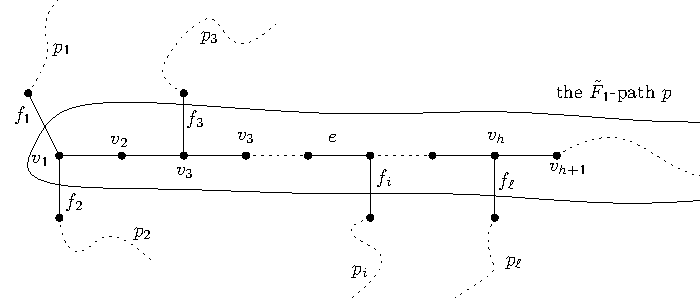
\includegraphics[width=.92\linewidth]{delayer-branches.pdf}\end{center}
Call $p_i$ blocked by $F_0$ if it contains some edge from $F_0$; at most $|F_0|$ of the $\ell$ paths are blocked by $F_0$. Let $p'$ be an $\widetilde F_1$-path different from $p$. We say $p'$ blocks $p_i$ if the vertex sets of $\phi(p')$ and $\phi(p_i)$ intersect.
\begin{authorclaim}{Proposition12}
Let path $p'$ in $\widetilde F_1$ be different from $p$. Then $p'$ blocks at most one of the paths $p_1,\ldots,p_\ell$.
\end{authorclaim}
\begin{proof}
Let $C=p\cup p_1\cup\cdots\cup p_\ell$. As argued above, this is a tree in $G$ and its diameter is less than $\operatorname{girth}(H)$. By Proposition11, its image $\phi(C)$ is a tree in $H$, isomorphic to $C$. Suppose, for the sake of contradiction, that $\phi(p')$ intersects $\phi(p_i)$ and $\phi(p_j)$. This scenario would look like this:
\begin{center}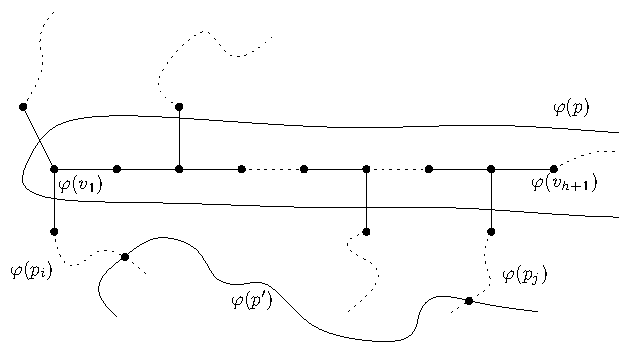
\includegraphics[width=.85\linewidth]{blocking-cycle.pdf}\end{center}
Since $\phi(p')$ and $\phi(p)$ do not share any vertex (by Invariant3), the subgraph $\phi(p')\cup\phi(p_i)\cup\phi(p_j)\cup\phi(p)$ contains a cycle. This cycle has size at most $|p'|+|p_i|+|p_j|+|q|\le2h\ell+2h+\ell+3h$, a contradiction.
\end{proof}
Call $p_i$ blocked by $\widetilde F_1$ if there is some $\widetilde F_1$-path different from $p$ that blocks $p_i$. By Proposition12, at most $|F_1|-1$ paths $p_i$ are blocked by $\widetilde F_1$. Thus, a total of at most $|F_0|+|F_1|-1\le\ell-1$ of the paths $p_i$ are blocked by $F_0$ or $\widetilde F_1$. Thus, there exists some path $p_i$, $1\le i\le\ell$, that is not blocked. We now modify $p$ by removing the edges on the path $v_1,v_2,\ldots,a_i$ and adding $p_i$. Let $\hat p$ denote the new version of $p$ and $\hat F_1$ the new version of $\widetilde F_1$. Note that $F_1\subseteq\hat F_1$ still holds, since we only modify the set $\widetilde F_1\setminus F_1$. Obviously, $\hat F$ satisfies Invariants1,2, and4. Since $p_i$ is not blocked by $F_0$, $\hat F$ is disjoint from $F_0$; because $p_i$ is not blocked by $\widetilde F_1$, Invariant3 still holds. Invariant5 might be violated: $\hat p$ might be too long. We will deal with this in a minute.
Note that $e$ is now either outside $\hat F_1$, and Delayer can include it into $F_0$; or it is inside $\hat p$, but then it is not among the first or last $h$ edges of $\hat p$, and Delayer can include it into $F_1$.
It remains to address the possibility that $\hat p$ is too long, violating Invariant5. If indeed $\hat p$ has more than $2h\ell+2h+\ell$ edges, then it must somewhere contain $2h+1$ consecutive edges that are not in $F_1$ (note that $|F_1|\le\ell$). Let $e_0,\ldots,e_{2h}$ be these edges. Define $\hat F_1:=\widetilde F_1\setminus\{e_h\}$. That is, we split $\hat p$ into two parts, the first ending in $e_0,\ldots,e_{h-1}$, the second starting with $e_{h+1},\ldots,e_{2h}$. Note that this satisfies Invariant4. If one of these paths contains no edge from $F_1$ at all, we delete it from $\hat F$. We continue this process until all paths in $\hat F$ have size at most $2h\ell+2h+\ell$. The final $\hat F$ satisfies all invariants.
